\documentclass[10pt, a4paper,spanish]{article}

\usepackage[utf8]{inputenc}
\usepackage[spanish]{babel}

\usepackage[T1]{fontenc}

\usepackage[hmarginratio=1:1,top=32mm,columnsep=20pt]{geometry}
\usepackage[hang, small,labelfont=bf,up,textfont=it,up]{caption}

\usepackage{float}

\usepackage{amsmath}

\usepackage{enumitem}

\usepackage{graphicx}
\graphicspath{ {images/} }


\usepackage{titlesec}
\renewcommand\thesection{\Roman{section}}
\renewcommand\thesubsection{\Roman{subsection}}
\titleformat{\section}[block]{\large\scshape\centering}{\thesection.}{1em}{}
\titleformat{\subsection}[block]{\large}{\thesubsection.}{1em}{}

\usepackage{fancyhdr}
\pagestyle{fancy}
\fancyhead{}
\fancyfoot{}
\fancyhead[C]{ \today \ $\bullet$ Ingeniería del Conocimiento $\bullet$ Clips 3}
\fancyfoot[RO]{\thepage}

%-------------------------------------------------------------------------------
%	TITLE SECTION
%-------------------------------------------------------------------------------

\title{\vspace{-15mm}\fontsize{24pt}{10pt}\selectfont\textbf{Clips 3}} % Article title

\author{
	Fernández Angulo, Óscar \\
	\and
	García Prado, Sergio
}

\date{\today}

%-------------------------------------------------------------------------------

\begin{document}

	\maketitle % Insert title

	\thispagestyle{fancy} % All pages have headers and footers


%-------------------------------------------------------------------------------
%	TEXT
%-------------------------------------------------------------------------------

	\section{Sistema Cardiovascular Humano Basado en Probabilidad}

		\begin{enumerate}

			\item Así, cuando un paciente se queja de un dolor abdominal, una auscultación permite percibir un rumor abdominal y al palpar el abdomen del paciente se siente una masa pulsante, un aneurisma de la arteria abdominal probablemente (0.8) cause estos síntomas y evidencias clínicas.

			\item Si la presión sistólica del paciente supera los 140 mmHg, la presión del pulso es superior a 50 mmHg, y al auscultar al paciente se percibe un rumor sistólico o una dilatación del corazón, todo ello puede estar causado por una regurgitación aórtica (0.7).

			\item Como último ejemplo, si un paciente siente calambres en las piernas al andar, que desaparecen tras uno o dos minutos de descanso, la presencia de una estenosis en una de las arterias de las piernas es más que probable (0.9). A su vez, la estenosis suele deberse a un problema de arteriosclerosis (0.8), especialmente si el paciente pertenece a algún grupo de riesgo: obeso (0.8) o fumador durante más de 15 años (0.8) o edad superior a 50 años (0.6).

		\end{enumerate}

		\subsection{Ontología General}

			\paragraph{}
			La base de conocimiento necesaria para representar el problema requiere de un conjunto tanto de objetos como de atributos de los mismos. Esto se describe a continuación a partir de la Definición del Dominio (DD) y el conjunto de reglas:

			\begin{multline*}
				O = \{ \\
					\{marta, luis, andres\} \in paciente, \\
					\{aneurisma\_arteria\_abdominal, regurgitacion\_aortica, \\
					estenosis\} \in enfermedad \\
				\}
			\end{multline*}

			\begin{multline*}
				DA = \{ \\
					paciente.genero^s:{hombre, mujer}, paciente.edad^s:number, \\
					paciente.sintomas^m, paciente.observacion^m, \\
					paciente.sistolica^s:number, paciente.diastolica^s:number, paciente.pulso^s:number, \\
					paciente.peso^s, paciente.fuma^s:number, paciente.diagnostico^m \\
				\}
			\end{multline*}


			\begin{enumerate}[label={\textbf{R\theenumi:}}]

				\item
					\textbf{if} $equals(?x, sistolica, ?y)$ \textbf{and} \\
						\hspace*{0.5cm} $equals(?x, diastolica, ?z)$ \\
					\textbf{then} $add(?x, pulso, (?y - ?z) )$ \textbf{fc} $1.0 $ \textbf{fi}
					\\ \\
					Calcula el pulso a partir del valor de la presión sistólica y diástólica del paciente.

				\item
					\textbf{if} $equals(?x, evidencia, rumor\_abdominal)$ \textbf{and} \\
						\hspace*{0.5cm} $equals(?x, evidencia, dolor\_abdominal)$ \textbf{and} \\
						\hspace*{0.5cm} $equals(?x, evidencia, masa\_pulsante\_abdomen)$ \\
					\textbf{then} $add(?x, diagnostico, aneurisma\_arteria\_abdominal)$ \textbf{fc} $0.8$ \textbf{fi}
					\\ \\
					Si el paciente tiene un rumor abdominal, dolor abdominal y una masa pulsante en el abdomen entonces sufre de un aneurisma en la arteria abdominal.

				\item
					\textbf{if} $greaterThan(?x, sistolica, 140)$ \textbf{and} \\
						\hspace*{0.5cm} $greaterThan(?x, pulso, 50)$ \textbf{and} ( \\
							\hspace*{1cm} $equals(?x, evidencia, rumor\_sistolico)$  \textbf{or}\\
							\hspace*{1cm} $equals(?x, evidencia, dilatacion\_corazon)$ \\
						\hspace*{0.5cm} ) \\
					\textbf{then} $add(?x, diagnostico, regurgitacion\_aortica$ \textbf{fc} $0.7$ \textbf{fi}
					\\ \\
					Si la presión sistólica del paciente es mayor que 140, su pulso que 50 y tiene un rumor sistólico o posee una dilatación en el corazón entonces el diagnóstico es un regurgitación aortical.

				\item
					\textbf{if} $equals(?x, peso, obeso)$ \\
					\textbf{then} $add(?x, diagnostico, estenosis)$ \textbf{fc} $0.8$ \textbf{fi}
					\\ \\
					Si el paciente tiene un peso elevado es un paciente de riesgo y por lo tanto podria tener estenosis con un alto grado de probabilidad.

				\item
					\textbf{if} $greaterThan(?x, fuma, 15)$ \\
					\textbf{then} $add(?x, diagnostico, estenosis)$ \textbf{fc} $0.8$ \textbf{fi}
					\\ \\
					Si el paciente fuma desde hace mas de 15 años es un paciente de riesgo y por lo tanto podria tener estenosis con un alto grado de probabilidad.

				\item
					\textbf{if} $greaterThan(?x, edad, 50)$ \\
					\textbf{then} $add(?x, diagnostico, estenosis)$ \textbf{fc} $0.6$ \textbf{fi}
					\\ \\
					Si el paciente tiene una edad mayor que 50 años es un paciente de riesgo y por lo tanto podria tener estenosis con un alto grado de probabilidad.

				\item
					\textbf{if} $equals(?x, sintomas, calambres\_pierna\_andar)$ \\
					\textbf{then} $add(?x, diagnostico, estenosis)$ \textbf{fc} $0.9$ \textbf{fi}
					\\ \\
					Si el paciente nota calambres en la pierna al caminar entonces pacede de estenosis.

				\item
					\textbf{if} $equals(?x, sintomas, arteriosclerosis)$ \\
					\textbf{then} $add(?x, diagnostico, estenosis)$ \textbf{fc} $0.8$ \textbf{fi}
					\\ \\
					Si el paciente tiene arteriosclrosis entonces pacede de estenosis con un alto grado de probabilidad.
			\end{enumerate}

		\subsection{Ontología Específica}

			\paragraph{}
			Los casos particulares que se pide codificar para conocer su diagnóstico se recogen en la siguiente tabla:

			\begin{figure}[H]
				\begin{center}
					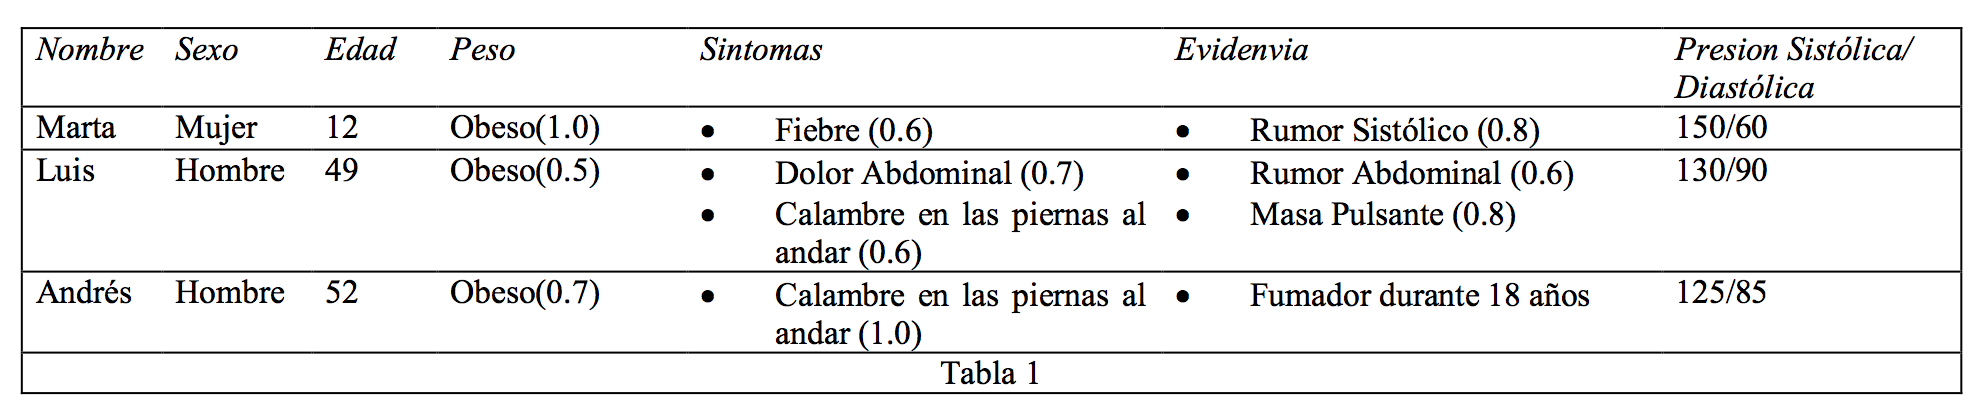
\includegraphics[width=\textwidth]{table-1}
				\end{center}
			\end{figure}

			\begin{equation*}
				\begin{split}
					marta.genero=mujer \ fc \  1.0 \\
					marta.edad=12 \ fc \  1.0 \\
					marta.peso=obeso \ fc \  1.0 \\
					marta.sintomas=\{fiebre \ fc \  0.6\} \\
					marta.observacion=\{rumor\_diastolico \ fc \  0.8\} \\
					marta.sistolica=150 \ fc \  1.0 \\
					marta.diastolica=60 \ fc \  1.0\\
					\\
					luis.genero=hombre  \ fc \  1.0 \\
					luis.edad=49  \ fc \   1.0 \\
					luis.peso=obeso \ fc \  0.5 \\
					luis.sintomas=\{dolor\_abdominal \ calambres\_pierna\_andar \ fc \  0.7 \ 0.6\} \\
					luis.observacion=\{rumor\_abdominal \ masa\_pulsante\_abdomen \ fc \  0.6 \ 0.8\} \\
					luis.sistolica=130 \ fc \  1.0 \\
					luis.diastolica=90 \ fc \  1.0 \\
					\\
					andres.genero=hombre \ fc \  1.0 \\
					andres.edad=52 \ fc \  1.0 \\
					andres.peso=obeso \ fc \  0.7 \\
					andres.sintomas=\{calambres\_pierna\_andar \ fc \  1.0 \} \\
					andres.observacion=\{fuma \ fc \  1.0\} \\
					andres.sistolica=125 \ fc \  1.0 \\
					andres.diastolica=85 \ fc \  1.0 \\
				\end{split}
			\end{equation*}



\end{document}
